\section{Evaluation}
\label{chap:evaluation}
Am Ende unserer Arbeit wurde uns ein Framework des SAFEST-Projekts zur Verfügung gestellt, dass die Möglichkeit bietet, verschiedene vorimplementierte Algorithmen mit einander zu vergleichen.\\
Nachdem wir unseren Algorithmus in das Framework integriert hatten, haben die folgenden Vergleiche mit einer vorimplementierten, Histogramm-basierten Lösung angestellt:
\begin{itemize}
	\item[a)] die vorimplementierte Lösung, die mit Histogrammen arbeitet
	\item[b)] unsere HMM-basierte Lösung mit generischen Werten für Initialwerte, Emission und Transition ohne Lernen
	\item[c)] unsere HMM-basierte Lösung mit generischen Werten für Initialwerte, Emission und Transition mit Lernen
\end{itemize}
Weitere Vergleiche haben wir nicht angestellt, da das Histogramm-basierte Verfahren den anderen Verfahren entweder überlegen ist (OpenCV MOG und OpenCV MOG2) oder aber das Verfahren den Hintergrund hart auf bestimmte Videos kodiert (MEAN) und sehr unflexibel ist, sobald der Hintergrund nicht mehr uniform ist.\\
Das Ergebnis haben wir jeweils visualisiert, indem wir für jeden zu evaluierenden Algorithmus die Abweichung vom eigentlich erwarteten Wert visualisiert haben.
Ein optimal funktionierender Algorithmus würde also als Bild im Diagramm ohne Abweichungen die Nulllinie verdecken.\\
Die erwarteten Werte für diesen Vergleich sind uns seitens des SAFEST Projekts zur Verfüngung gestellt worden.
\subsection{Vergleich mit Histogramm-basierter Implementierung: Innenhof}
\label{sec:eval_innenhof}
\begin{figure}
	\centering
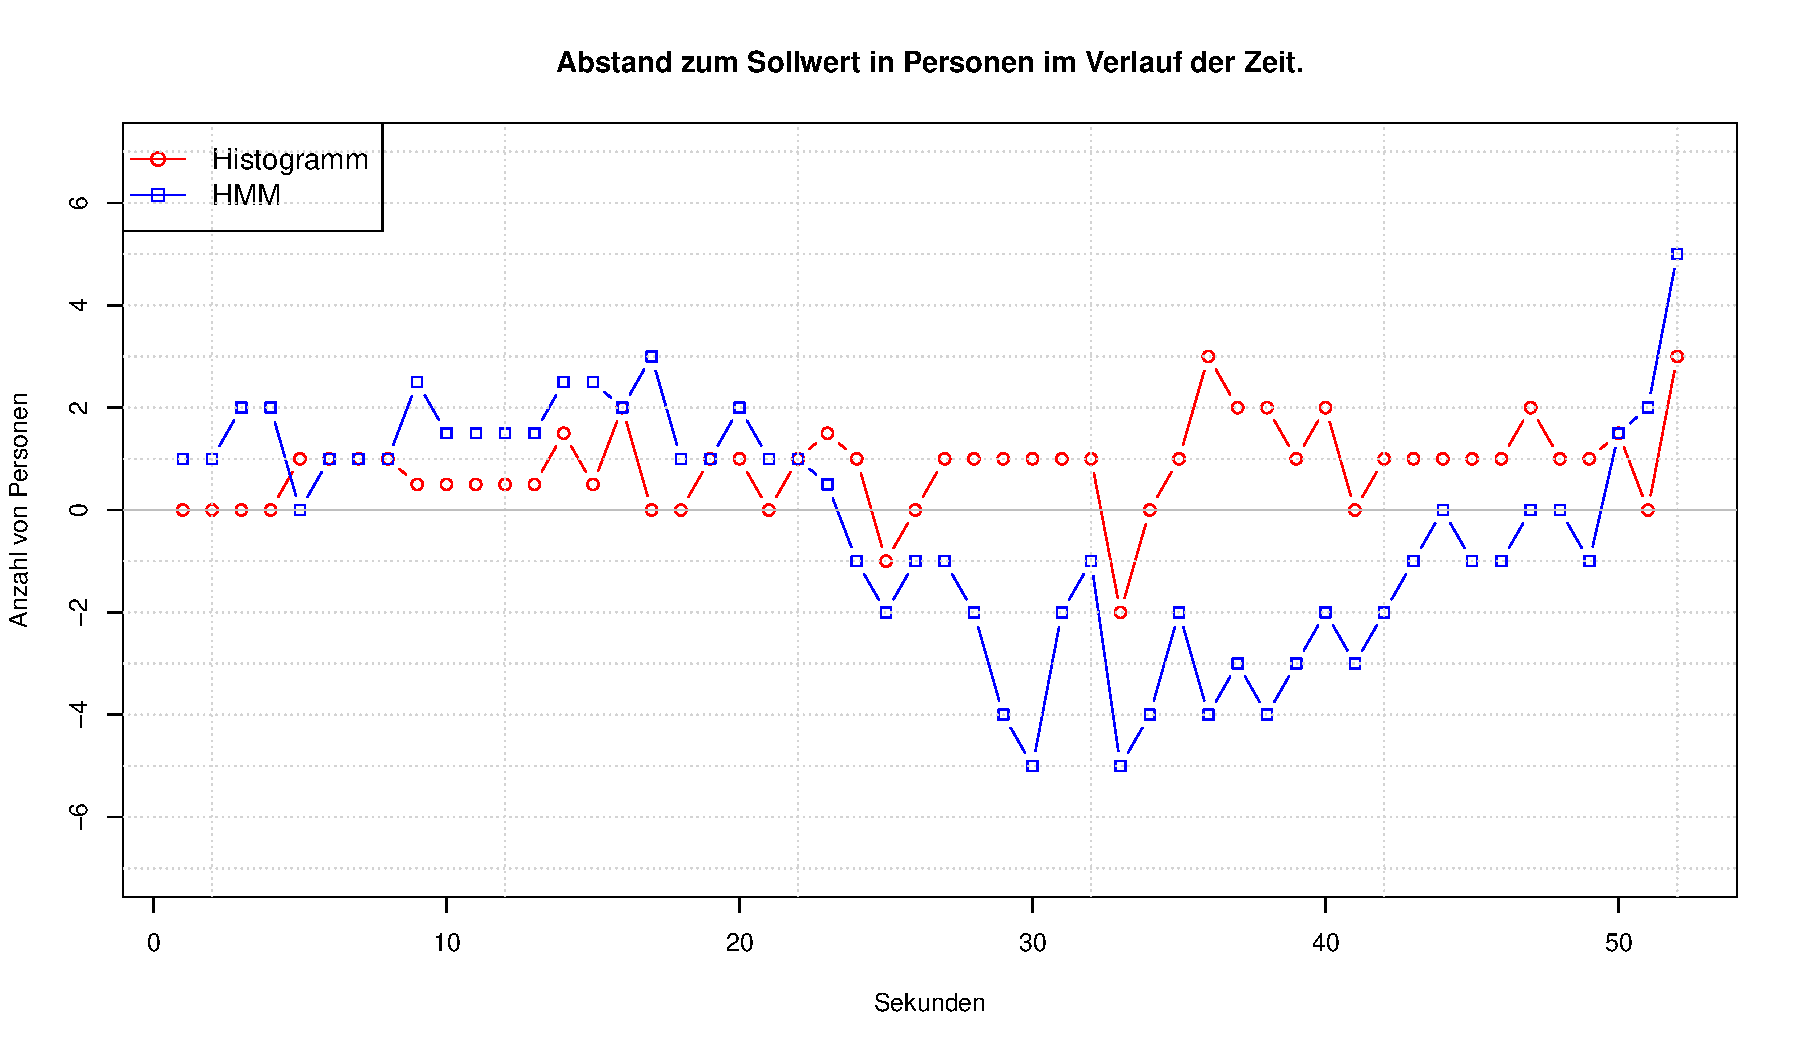
\includegraphics[width=1\textwidth]{bilder/innenhof_910-1000_histo_vs_hmm_prelearned.pdf}
\caption{Innenhof: Histogramm vs. trainiertes HMM}
	\label{fig:Innenhof}
\end{figure}
In Grafik \ref{fig:Innenhof} sieht man, dass der Histogramm-basierte Algorithmus für dieses Video bessere Ergebnisse liefert, als der HMM-basierte Algorithmus.\\

\subsection{Vergleich mit Histogramm-basierter Implementierung: Tegel}
\label{sec:eval:tegel}
\begin{figure}
	\centering
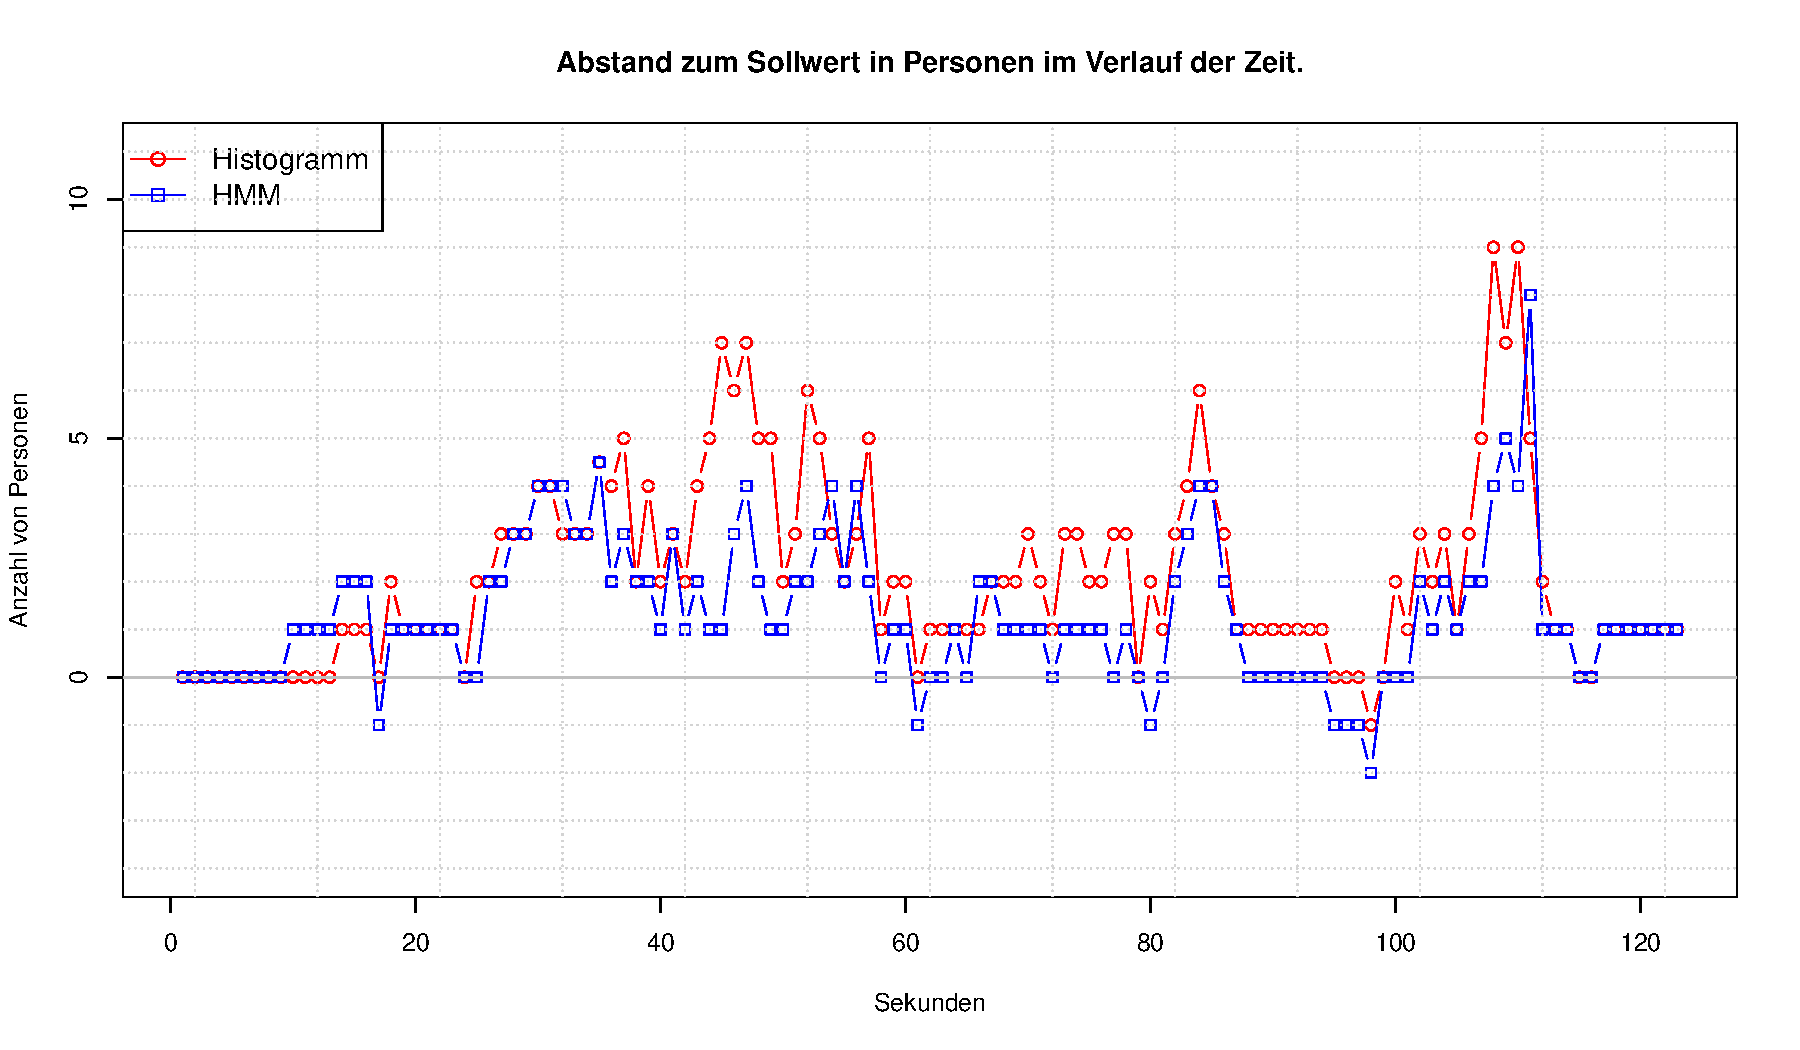
\includegraphics[width=1\textwidth]{bilder/tegel_7-55_histo_vs_prelearned_hmm.pdf}
	\caption{Tegel: Histogramm vs. trainiertes HMM}
	\label{fig:tegel}
\end{figure}

Wie man Abbildung \ref{fig:tegel} entnehmen kann, sind die Ergebnisse beider Algorithen vom Verlauf her sehr ähnlich.
Allerdings hat der HMM-basierte Algorithmus gegenüber dem Histogram-basierten kleine Vorteile.
Zwischen 30 und 50 Sekunden hat er eine deutlich geringere Abweichung vom korrekten Wert.
Dasselbe gilt für den Bereich zwischen ca. 65 und 80 Sekunden.\\
Insgesamt kann man aber sagen, dass am überraschensten ist, wie ähnlich der Verlauf der beiden Graphen ist. Zum Teil ist dies sicher darauf zurückzuführen, dass der Clustering-Algorithmus in beiden Fällen nicht richtig gut funktioniert.

\subsection{Vergleich mit Histogramm-basierter Implementierung: Eingang}
\label{sec:eval_eingang}
\begin{figure}
	\centering
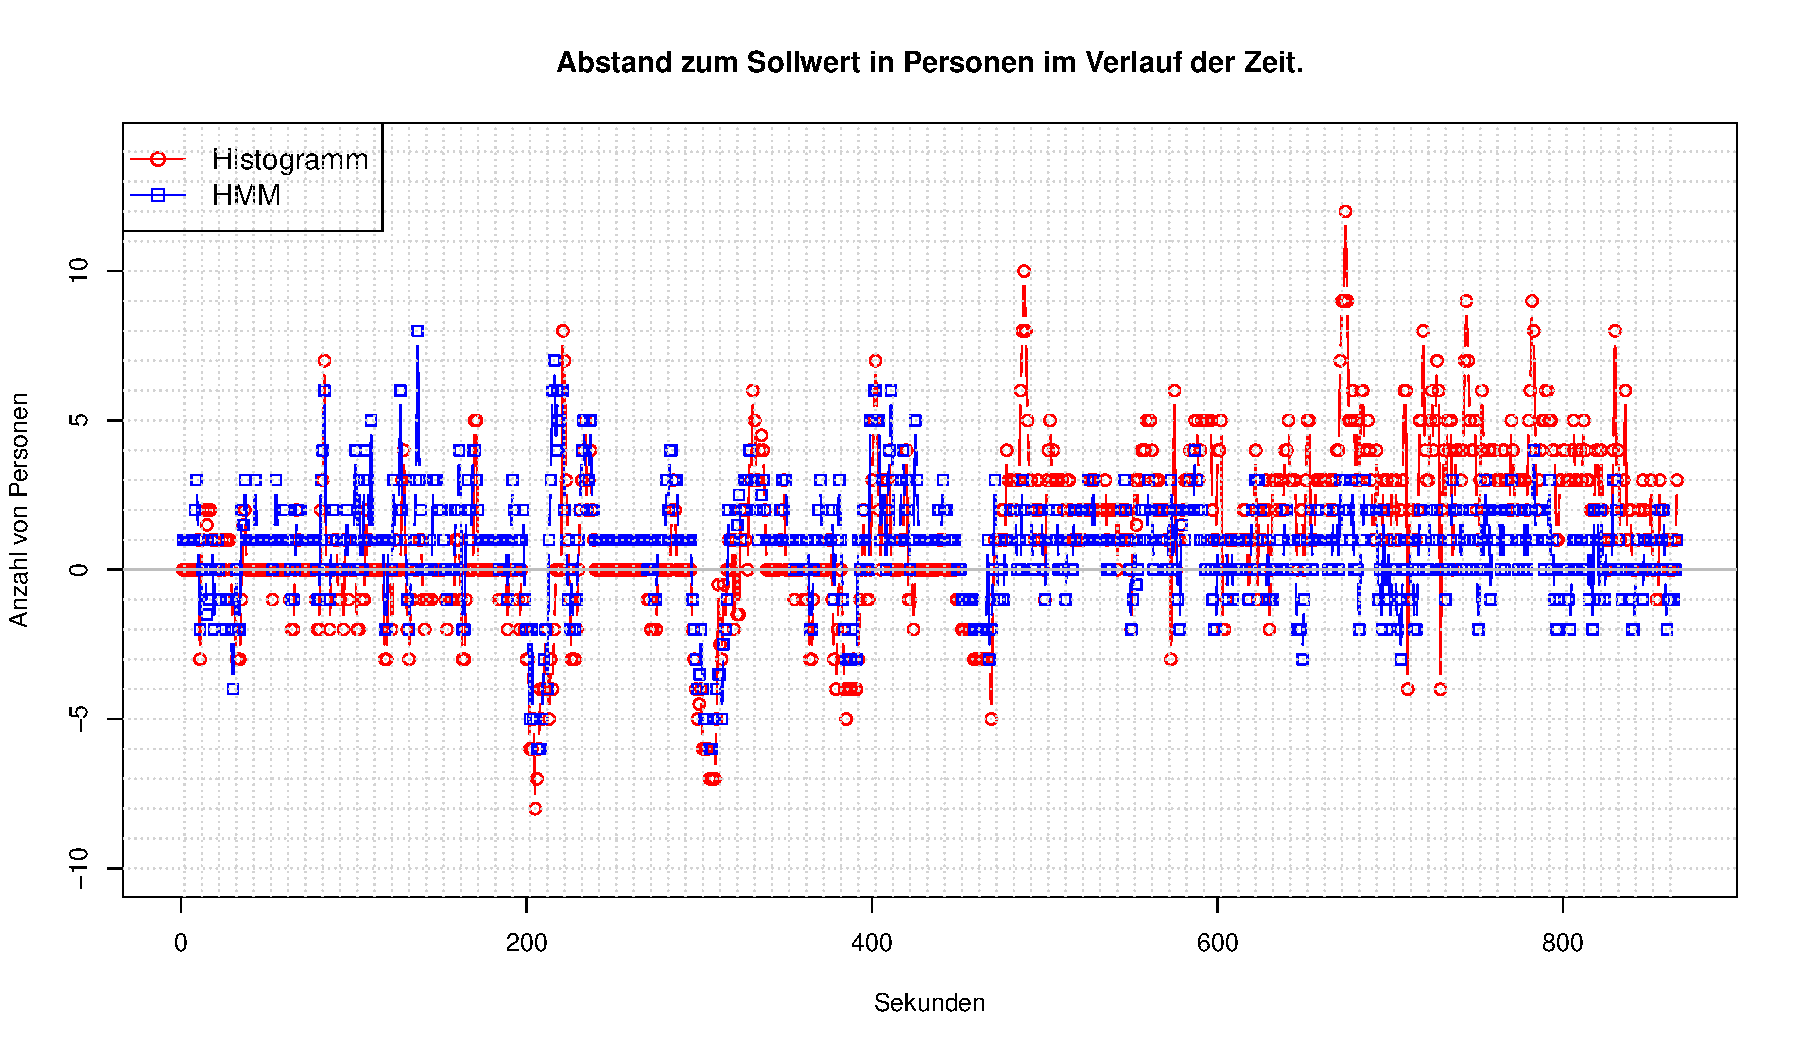
\includegraphics[width=1\textwidth]{bilder/eingang2_histo_vs_hmm_prelearned.pdf}
\caption{Eingang: Histogramm vs. trainiertes HMM (gesamt)}
	\label{fig:Eingang-gesamt}
\end{figure}
\begin{figure}
	\centering
	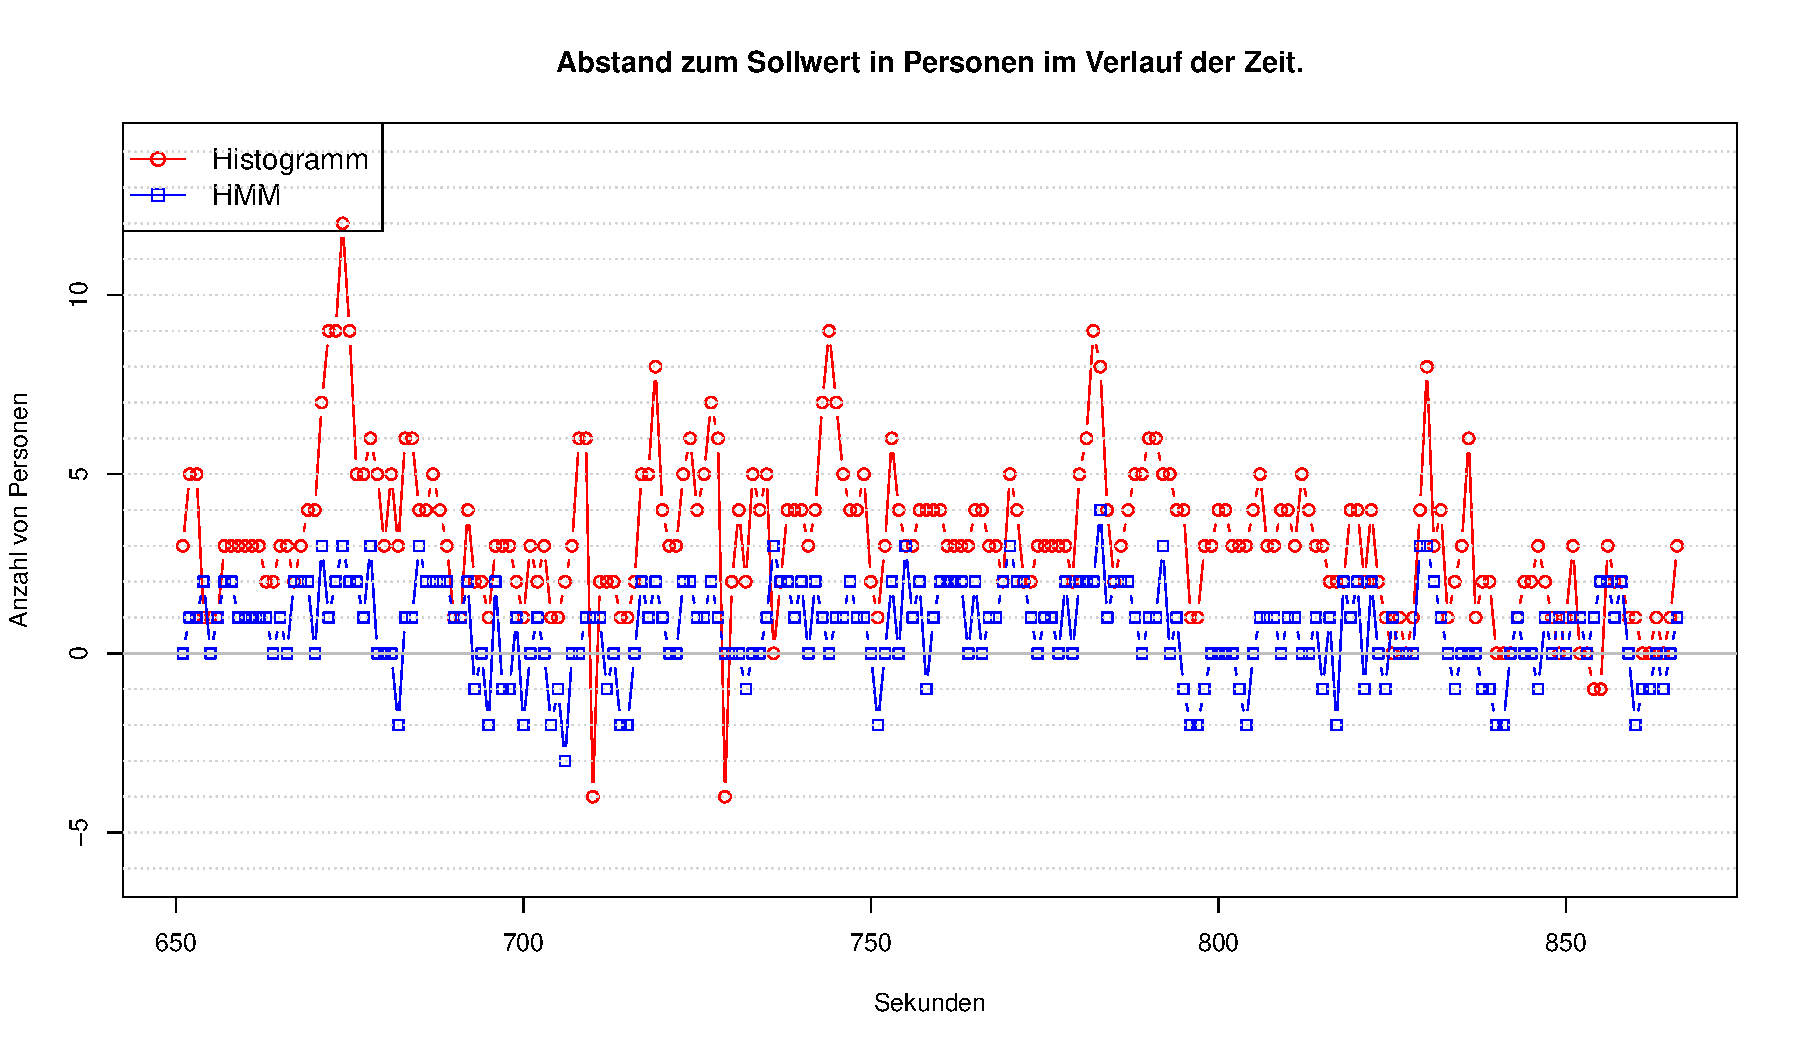
\includegraphics[width=1\textwidth]{bilder/safest_plot_histo_vs_prelearned_652-end.pdf}
	\caption{Eingang: Histogramm vs. trainiertes HMM, Auschnitt Frame 651-Ende}
	\label{fig:Eingang-teil}
\end{figure}
In der Grafik \ref{fig:Eingang-gesamt} sieht man, dass beide Algorithmen hier nicht wirklich gut funktioieren.
Dies ist aufgrund der Eigenschaften des Videos zu erwarten: der Hintergrund ist sehr hell und die Kalibrierung der Kamera fällt hier auch optisch sehr stark auf.\\
Während in der ersten Hälfte des Videos der Histogramm-basierte Algorithmus noch Vorteile hat (relativ viele korrekte Anzeigen, der HMM-basierte Algorithmus erkennt meist eine Person zu viel). ist der HMM-basierte Algorithmus in der zweiten Hälfte des Videos (ab etwa Frame 450) deutlich besser.
in Grafik \ref{fig:Eingang-teil} sieht, gibt es wesentlich weniger Ausreißer und das Ergebnis ist insgesamt auch viel dichter am korrekten Wert.\\
Wie auch im Falle der Tegelvideos liegt der Fehler aber auch hier daran, dass der Clustering Algorithmus häufig einen Menschen in mehrere Cluster teilt, weil er nicht gut genug an das Video angepasst ist. Wenn man den Clustering-Algorithmus entsprechend anpassen würde, so dass eine Mensch nicht mehr in 2-4 Cluster geteilt wird, würde der HMM-basierte Algorithmus in der zweiten Hälfte des Bildes vermutlich sehr dicht am korrekten Wert liegen.

\subsection{Diskussion}
\label{sec:diskuss}

Zu erkennen an den beschreibung der vorangehenden graphiken ist das....

%TODO:
 %bezug auf anforderungen nehmen, punkte erfüllt?
 %hmm topologie?
 %andere libs?
 %forward vs. viterbi
 %dynamische histrogramm/cluster grenzen für dc wert in zukunft?
 %viterbi/forawrd gibt zustand, man kann entweder gewichtestes würfeln oder aber deterministisch die wahrschienlichste beobachtung nehmen, was ist besser? -> test?
 %performance gewinn durch threading zusätzlich
Lerndauer vermutlich zu kurz, daher stellt sich das HMM nie richtig ein und es kommt zusätzlich zu Effekten wie Ghosting.

Der Vergleich der Algorithmen bezieht sich rein auf das Ergebnis der Hintergrder Algorithmen bezieht sich rein auf das Ergebnis der Hintergrundentfernung.
Im Bezug auf Performance ist der Histogramm-basierte Algorithmus wesentlich besser (ca. 3-4 Frames/sec vs. ca 20-25 Frames / sec).

Größte Performance-Bremse lt. Callgrind: der .at(foo, bar): Zugriff auf einzelne Elemente des Arrays.

\subsection{CvHMM}
\label{sec:CvHMM}
Leider hat sich im Laufe des Projekts gezeigt, dass CvHMM leider sehr ineffizient auf einzelne Daten zugreift.\\

Ein weiterer großer Nachteil von CvHMM ist, dass nur der Baum-Welch-, der Viterbi- und der Decode-Algorithmus angeboten werden.
 Gerade hier ist wiederum ein Manko zu sehen, da wir später den Forward-Algorithmus gebraucht hätten und nun stattdessen den Viterbi-Algorithmus verwenden müssen, der jedoch ineffizienter als der Forward-Algorithmus ist.

Zusammenfassend lässt sich zur Wahl der HMM Bibliothek sagen, dass es wohl das Ergebnis des Projekts erheblich hätte verbessern können, wenn unsere Wahl auf eine andere Bibliothek gefallen wäre.

Mögliche Kandidaten zum Testen wären dabei HMMlib oder vielleicht sogar die, wie wir später herausgefunden haben, in OpenCV enthaltenen HMM-Funktionen, die allerdings innerhalb des OpenCV-Projekts nicht weiterentwickelt werden und derzeit des Status “deprecated” haben.
